\documentclass[11pt,a4paper]{article}

\usepackage{graphicx}
\usepackage{tabularx}
\usepackage{subfigure}
\usepackage{afterpage}
\usepackage{amsmath,amssymb}            
\usepackage{rotating}  
\usepackage{fancyhdr}  
\usepackage{cite}
%\usepackage[scriptsize]{caption2} 
\hyphenation{a-gen-tiz-za-zio-ne}

\setlength{\paperwidth}{16cm}
\setlength{\paperheight}{24cm}
\setlength{\oddsidemargin} {2. cm}
\setlength{\evensidemargin} {2. cm}
\addtolength{\oddsidemargin} {-0.4 cm}
\addtolength{\evensidemargin} {-0.4 cm}
\linespread{1.1}

\usepackage[english]{babel}
\usepackage[latin1]{inputenc}
%\renewcommand{\captionfont}{\normalfont \sffamily \itshape \small}

\pagestyle{empty}



\begin{document}
\thispagestyle{empty}
%\begin{titlepage}
\vspace*{-1.5cm} 
\begin{center}
  \large
  POLITECNICO DI MILANO\\
  \normalsize
  Alta Scuola Politecnica\\
  \begin{figure}[htbp]
    \begin{center}
      
\includegraphics[width=5.5cm]{../img/logoasp.png}
	%
\psfig{file=./pictures/logopm.jpg,width=3.5cm}
    \end{center}
  \end{figure}
  \vspace*{0.3cm} \LARGE



  \textbf{Polygame: developer guide}\\



  \vspace*{.75truecm} \large
  Spring School 2009 \\
  V Cycle \\
  Global change and sustainability\\
  Barbara Betti, Stefano Consonni, Marino Gatto
  
 % AI \& R Lab \\
 % Laboratorio di Intelligenza Artificiale \\
 % e Robotica del Politecnico di Milano
\end{center}
\vspace*{2.0cm} \large
\begin{flushleft}


  %Relatore: Ing. Matteo Matteucci \\
  %Correlatore: Prof. Andrea Bonarini 

\end{flushleft}
%\vspace*{1.0cm}
\begin{flushright}


  Mario Sangiorgio\\Computer Engineering\\ \emph{mario.sangiorgio@asp-poli.it} \\ 
      %Marco Triverio\\Computer Engineering\\marco.triverio@asp-poli.it \\ 


\end{flushright}
%\vspace*{0.5cm}
\begin{center}



  %Anno Accademico 200N-200N+1
\end{center} \clearpage

%\thispagestyle{empty} \normalfont \cleardoublepage
%\include{dedica}
%\thispagestyle{empty}  \cleardoublepage
%\pagenumbering{Roman}
%\include{sommario}
%\thispagestyle{empty} \vspace*{.75truecm} \cleardoublepage
%\include{ringraziamenti}
%\thispagestyle{empty} \vspace*{.75truecm} \normalfont \cleardoublepage
%\pagestyle{plain}

\tableofcontents
%\pagestyle{empty}\cleardoublepage
\pagenumbering{arabic}

\pagestyle{fancy} 
\fancyfoot{}                                               
%\renewcommand{\chaptermark}[1]{\markboth{\chaptername\ \thechapter.\ #1}{}} 
\renewcommand{\sectionmark}[1]{\markright{\thesection.\ #1}}         
\fancyhead[LE,RO]{\bfseries\thepage}    
                                        
\fancyhead[RE]{\bfseries\leftmark}    
\fancyhead[LO]{\bfseries\rightmark}     
\renewcommand{\headrulewidth}{0.3pt} 

\section{Introduction}
This document is the developer guide to the \emph{polygame} project. The goal of this project is to provide a easy to use interface to play a game to increase the knowledge about the topic of sustainability and how it is possible to make the current \emph{$CO_2$} emission situation better.


The game idea comes from the work of Robert H. Socolow and Stephen W. Pacala described in \cite{scientificAmerican} and \cite{science}.

This project is based on the game proposed by professors Renato Casagrandi and Giulia Fiorese in the ASP Spring School 2009, as an activity for the course \emph{Global Change and Sustainability}

In this game students first have to study a single environmental topic, to find out the effort needed to reduce the related \emph{$CO_2$} emissions by 1 MegaTon. Each student or each group of students will be assigned to study a different topic to have all the possible issues covered by the class.

When the study part is over, students have to present to the class what are the result they obtained, pointing out what are the point of strength and the weakness of the proposed solution. From  the case they studied and the presentation of their class-mates, students should have a basic knowledge about all the topics.

In the second phase of the game students are asked to apply what they have just learned to create a plan to reduce the emissions by at least 20 MegaTons, using a combination of the solution studied before.

At the end of this phase students will present their environmental plan to the class, giving a brief overview of it and explaining the reasons of the choices.

The proposed plan as well as its presentation will be used by a panel of voters to decide the winner of the game

With \emph{polygame} we provide a web application that makes it easier to play the game in all its phases, making all the needed material available to the students and helping the organizer to follow what is going on.

In the next section of this document the technologies used to implement the application will be discussed and some implementation details will be provided to help the reader understanding how it works.
\section{Rules of the game}
\label{rules}
The aim of this game is to gain a good understanding of the possible technologies that can reduce CO$_{2}$ emissions and to be able to come up with a good mix of those to act against the climate crisis.\\

Players can either take part in the game singularly or in a group. In both cases the game is divided in two phases:
	\begin{description}
		\item[Phase one] It is the phase of the game when every single user and every group is assigned to a certain \emph{wedge}. A \emph{wedge} is a certain solution which can reduce CO$_{2}$ emissions by 1 MegaTon. Every group and every single user has to investigate the given wedge in order to find out pros and cons. At the end of this phase the group or the single user has to outline all the pros and cons in a \emph{poster}, which should be described in front of the audience in a few minutes (the exact number of minutes is decided by the organizer). The purpose of the presentation is to make everybody aware of the possible solutions to reduce CO$_{2}$ emissions.
		\item[Phase two] After the first phase every user might be assigned to a new group (while there might still be single user). Groups of phase two do not work a specific wedge but they have to come up with the best possible \emph{plan} to reduce emissions using a mix of the wedges studied in the previous phase. The minimum reduction of CO$_{2}$ should be at least be 20 MegaTons so a minimum quantity of 20 wedges is required. Any wedge can be selected more than once and this allows a wide range of possible solutions (and also a wide margin for discussion).
	\end{description}
	
	 At the end of phase two plans are voted and the most voted becomes the \emph{winner} of Polygame.\\
All comments left by voters to the voters are displayed.
\section{Users roles}
\label{users}

Polygame features different kind of users:
\begin{itemize}
	\item Players
	\item Organizers
	\item Voters
	\item Administrators
\end{itemize}

One by one these roles will be explained in the next sections.
An overview of the roles is shown in the following figures
  \begin{figure}[htbp]
    \begin{center}
      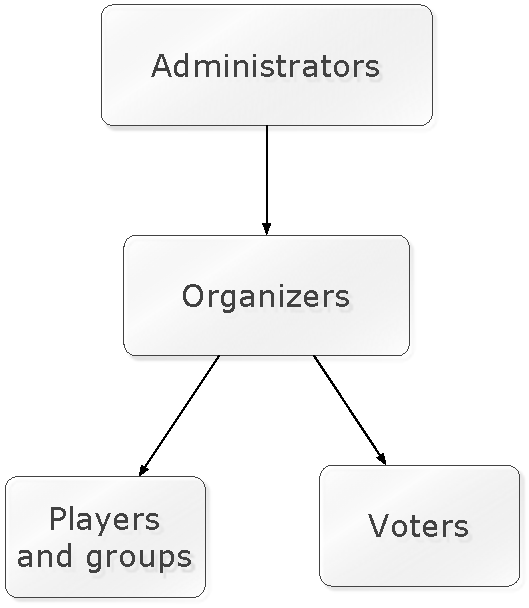
\includegraphics[width=8cm]{../img/Users.pdf}
	%
\psfig{file=./pictures/logopm.jpg,width=3.5cm}
    \end{center}
  \end{figure}

\subsection{Players}
\subsubsection{Introduction}
Those are the most common users and are the ones who take part in the game. They are provided a password by the organizers.		
Players can take take part in the game in two different ways:
\begin{itemize}
	\item singularly
	\item as part of a group
\end{itemize}
There are two different kinds of groups:
\begin{itemize}
	\item groups of first phase or groups that study a certain wedge
	\item groups of second phase or groups that have to come up with a plan (choice of wedges)
\end{itemize}
Our web application provides maximum flexibility because a user can be part of different groups in different phases and, if needed, can compete singularly in either one or both phases.

\subsubsection{Game}
After logging in the user is presented with a web page which is dynamically updated depending on the current phase of the game.\\
Those are the possible phases:
\begin{description}
	\item[Game not started] The user is presented with the rules of the game and is warned that the game is not started
	\item[Phase 1 just started] This phase is also known as \emph{Wedge introduction} and it is the first phase of the game. The player is presented the topic regarding the wedge and she or he is given time to find a little more information about the topic.
	\item[Central part of phase 1] This phase is also known as \emph{Wedge description} and it is the phase in which the player is provided with a more detailed description of the wedge. He or she is also provided with a PDF presenting data regarding all the wedges. The player is required to find the more interesting ones and use them to calculate the solution that he or she will have to enter in the following phase. 
	\item[Last part of phase 1] This phase is also known as \emph{Wedge solution and plan}. In this phase the player (either singularly or as part of a group) is given the chance to enter:
	\begin{itemize}
	\item the numeric solution to the problem presented in the previous phase
	\item the poster which should summarize what has been found out about the given wedge. In particular he is given the chance to:
	\begin{itemize}
\item enter pros
\item enter cons
\item enter additional notes
\end{itemize}
\end{itemize}

	\item[Poster presentation] When phase one is over, a break is started. In such break every group (or every single user) is given a few minutes to present the developed poster in front of the audience. For more information about this, please see the Organizer section.\\
	\item[Wedge plan creation] When the organizer decides so, the second phase is started and, if needed, the player is assigned to a new group. In this second phase the player (possibly along with her or his group-mates) has to come up with a plan to reduce emissions. In this phase users have access to the posters previously created. To summarize the reasons why players have chosen a certain mix of wedges, they are asked to create a short presentation of their solution: such short presentation will be available to voter and will certainly play an important role in their decision.
	\item[Plan choice] After the game is ended, voters can pick their favorite plan. The plan which gets the more votes is then shown on the organizer page.
\end{description}

\subsection{Organizers}
\subsubsection{Introduction}
Organizers are a central kind of user: they are the creators of the game and for this reason they have a wide range of possible choices.\\
As for the players, organizers are presented with a webpage whose content changes depending on the current phase of the game.\\
Administrators provide the password to the organizers.

\subsubsection{Game}
The organizer has total control over the game: after creating the game she or he can start the game, can move between game phases, assign more time to a phase and end the game prematurely.
\begin{description}
	\item[Game not created] After logging in the organize is given the possibility of creating a new game. At this point she or he can choose several parameters of the game:
		\begin{itemize}
		\item Timeout before more information about the wedge are provided
		\item Timeout before the players are allowed to submit a solution
		\item Timeout before the players are allowed to submit (and, in case, edit) the poster
		\item Time provided for one poster presentation
		\item Time provided to come up with a plan to reduce emissions
		\end{itemize}
	\item[Game not started] In this phase the organizer can:
		\begin{itemize}
		\item Handle players creating new players, deleting them from the database, adding them to the game and removing them from the game
		\item Handle wedges, choosing the ones which should be part of the game. Please note that the number of wedges should equal the sum of the number of groups of the first phase and singular users
		\item Handle groups, creating new groups and selecting which players should be part of which group
		\item Handle voters creating new voters, deleting them from the database, adding them to the game and removing them from the game
		\end{itemize}	
	\item[Phase 1] After clicking on start game the organizer is always shown controls to move between phases and to assign more time to a phase. Moreover during all phase one the organizer is shown a table which summarize the status of the game. In particular the table shows, for every single player and every group:
	\begin{itemize}
		\item the name of the single player or the name of the group
		\item whether they have attempted to provide a solution
		\item whether the solution is correct
		\item whether a poster has been submitted
		\item whether the submitted poster is complete (it has both pros and cons)
	\end{itemize}
	\item[Poster presentation] The poster presentation phase is entirely handled by the organizer, who chooses the poster to shown and provides a fixed amount of time to the presenter. After the time is elapsed the poster disappears.
	\item[Phase 2] After clicking on ``start phase two'' the organizer is shown a table which summarize the status of the current phase. In particular the table shows, for every single player and every group:
	\begin{itemize}
		\item the name of the single player or the name of the group
		\item whether they submitted a plan or not
	\end{itemize}
	\item[Voting phase] After the game ends and after all voters have provided their opinion, the organizer page shows the results of the voting. Please note that only the winner is shown and that comments provided to that plan are also shown.
\end{description}
    \begin{figure}[htbp]
    \begin{center}
      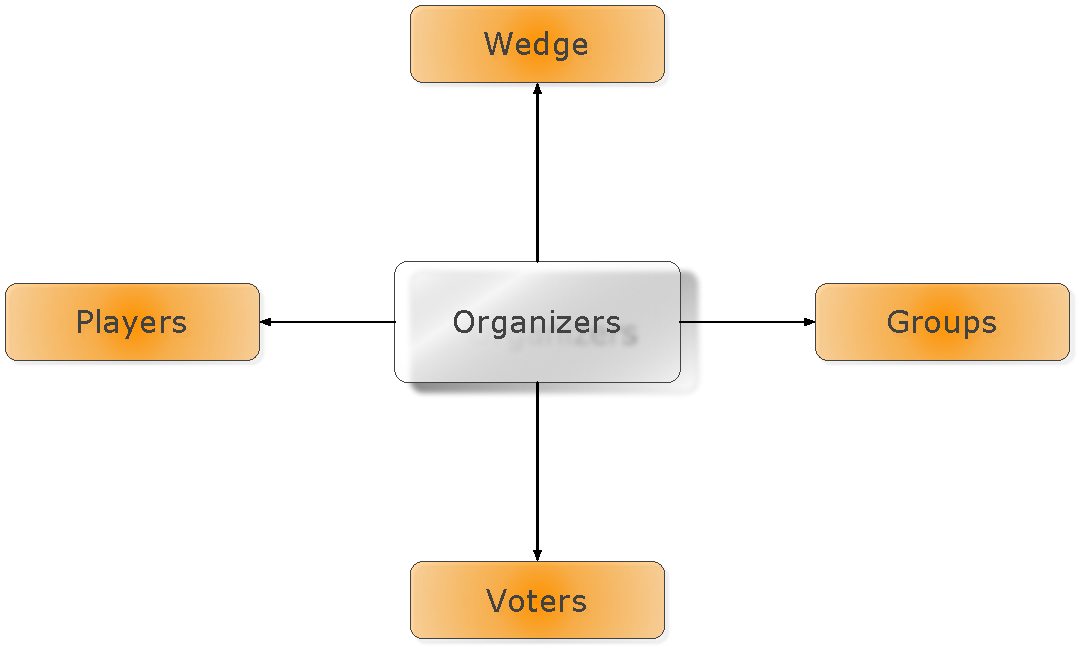
\includegraphics[width=12cm]{../img/Organizer.pdf}
	%
\psfig{file=./pictures/logopm.jpg,width=3.5cm}
    \end{center}
  \end{figure}

\subsection{Voters}
Voters are created and chosen by the organizer. Their role starts right after the game ends. They are provided with a page that summarizes all the plans. For each plan a link to the presentation (which summarizes the reasons that have led to a certain plan) is also provided. Voters can pick the one and only one plan they prefer. Additionally they can also provide a comment.\\
Only comments referring to the winner plan will be shown (on the organizer's page).

\subsection{Administrators}
Administrators do not handle game as the organizers but they handle some core functionalities of the game. They can:
	\begin{itemize}
		\item create new organizers providing a username and a password
		\item create new wedges, which might be later selected by organizers for their own game
	\end{itemize}
  
  
  
%\include{capitolo4}
%\include{capitolo5}
%\include{capitolo6}
%\include{capitolo7}

\clearpage
% ---- Bibliography ----
\addcontentsline{toc}{section}{Bibliography}
\bibliographystyle{plain}
\bibliography{bibl_tesi}
%\nocite{*}

\appendix

\pagestyle{fancy} 
\fancyfoot{}                                               
%\renewcommand{\chaptermark}[1]{\markboth{\appendixname\ \thechapter.\ #1}{}} 
\renewcommand{\sectionmark}[1]{\markright{\thesection.\ #1}}         
\fancyhead[LE,RO]{\bfseries\thepage}    
                                        
\fancyhead[RE]{\bfseries\leftmark}    
\fancyhead[LO]{\bfseries\rightmark}     
\renewcommand{\headrulewidth}{0.3pt} 

\end{document}





